
\lettrine[lines=3]{T}{he} process of generating WebAssembly binaries starts with the original source code, which is then processed by a compiler to produce a \Wasm binary. 
This compiler is generally divided into three main components: a frontend that converts the source code into an intermediate representation, an optimizer/transformer that modifies this representation usually for performance, and a backend that compiles the final \Wasm binary.
This architecture is illustrated in the leftmost part of \autoref{fig:approach_landscape}.

\begin{figure}[h]
	\centering
	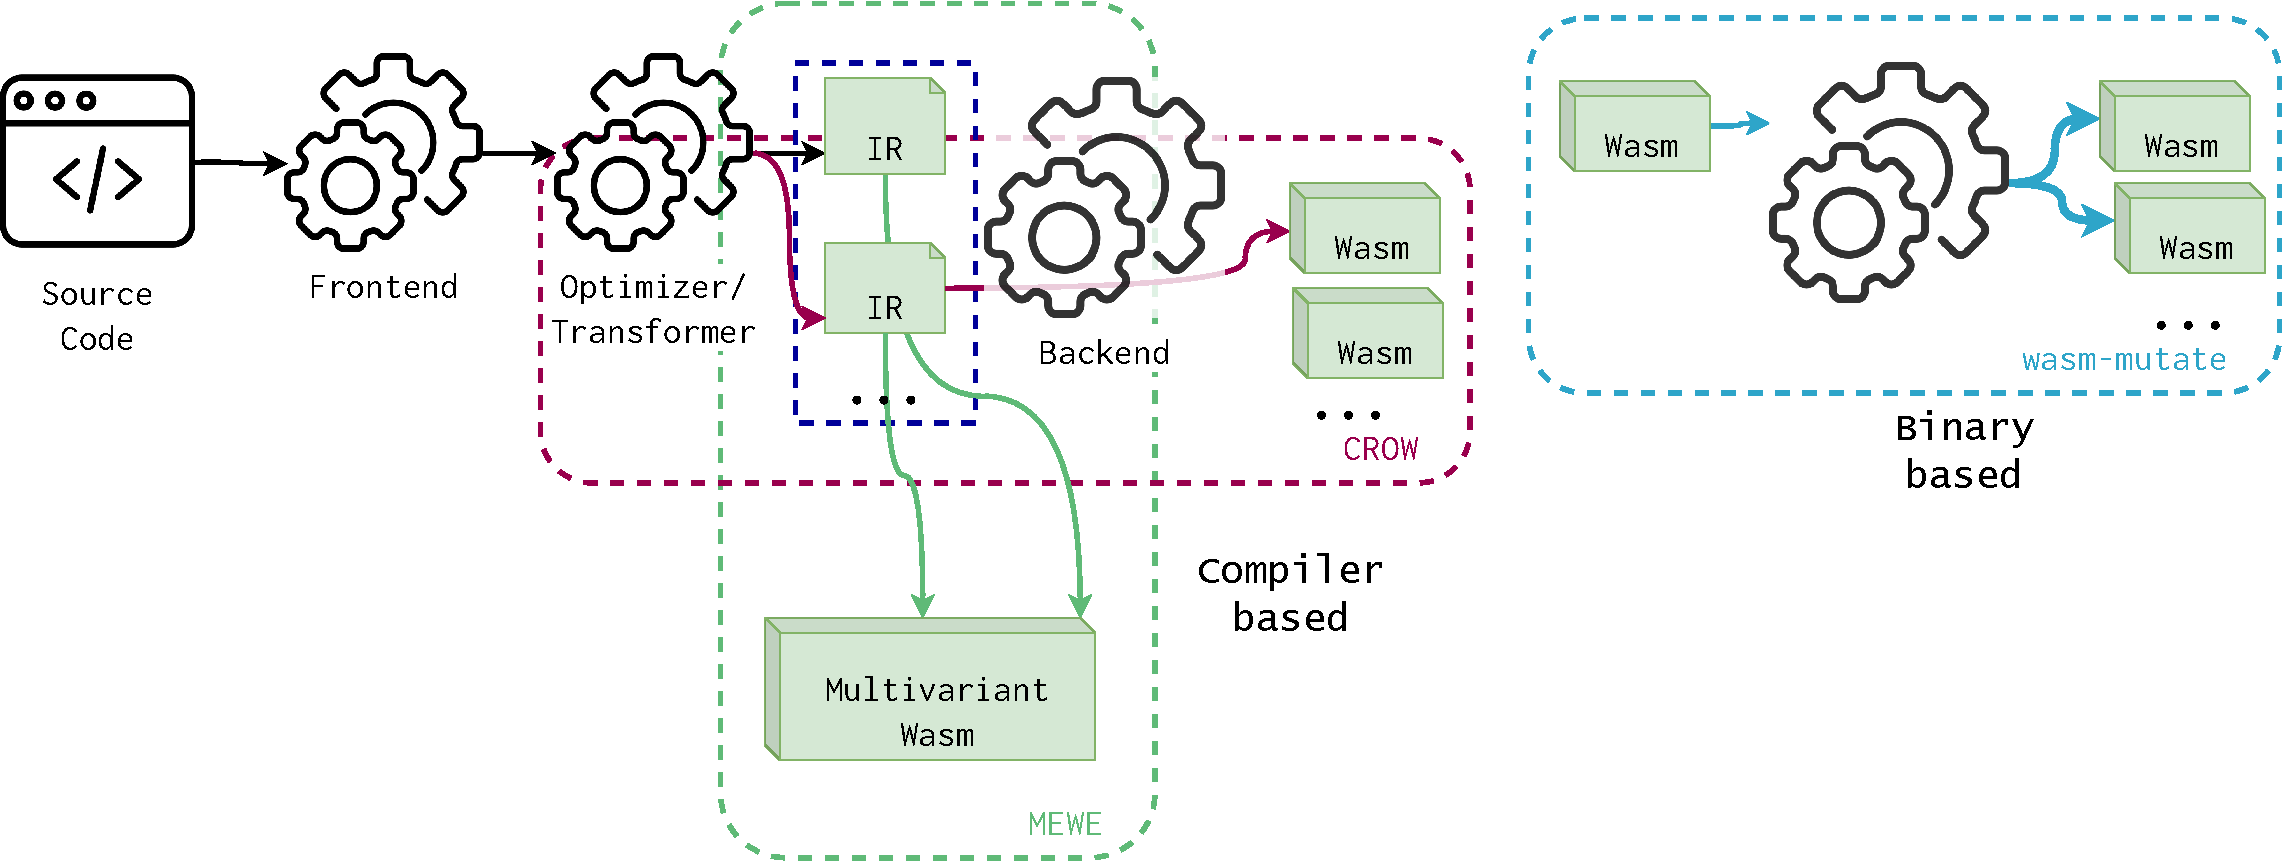
\includegraphics[width=0.9\textwidth]{figures/landscape.pdf}
	\caption{Approach landscape containing our three technical contributions: CROW squared in red, MEWE squared in green and WASM-MUTATE squared in blue. We annotate where our contributions, compiler-based and binary-based, stand in the landscape of generating \Wasm programs.}
	\label{fig:approach_landscape}
\end{figure}

Software Diversification can be integrated at various stages of this compilation process. 
However, applying diversification at the frontend has limitations, as it would need a unique diversification mechanism for each language compatible with the frontend component. 
Diversification at later compiler stages, such as the optimizer or backend, offers a more practical alternative.
This makes the latter stages of the compilers an ideal point for introducing practical \wasm diversification techniques.
Our compiler-based strategies, represented in red and green in \autoref{fig:approach_landscape}, introduce a diversifier component into the optimizer/transformer and backend stages. 
This optimization/transformer component generates variants in the intermediate representation of a compiler, thereby creating artificial software diversity for \Wasm. 
The variants are then compiled into \Wasm binaries by the backend component of the compiler.
Specifically, we propose two tools: CROW, which generates \Wasm program variants, and MEWE, which packages these variants to enable multivariant execution \cite{cox06}.
Alternatively, diversification can be directly applied to the \Wasm binary, offering a language and compiler-agnostic approach. 
Our binary-based strategy, WASM-MUTATE, represented in blue in \autoref{fig:approach_landscape}, employs rewriting rules on an e-graph data structure to generate a variety of \Wasm program variants.

This dissertation contributes to the field of Software Diversification for \Wasm by presenting two primary strategies: compiler-based and binary-based. 
Within this chapter, we introduce three technical contributions: CROW, MEWE, and WASM-MUTATE.
We also compare these contributions, highlighting their complementary nature.
Additionally, we provide the artifacts for our contributions to promote open research and reproducibility of our main takeaways.


\renewcommand{\tool}{CROW\xspace}